In the next section, we present our results obtained by full frequency dependent fRG. All the results are presented in units of $t=1$.  
\paragraph*{Numerical implementation}
We have implemented numerically the flow equations reported in the appendix. 
Due to the different nature of the momentum arguments of self-energy and vertex we have defined two different patching schemes of the irreducible Brillouin zone. 
%The $\phi$-functions depend on a momentum transfer.  
%For the filling and nearest neighbors hopping that we want to describe, the momentum vectors of the most relevant process are $\mathbf{Q}=(0,0)$, important for superconductivity (in the pairing channel) and ferromagnetism (in the magnetic channel); $\mathbf{Q}=(\pi,\pi)$ and its vicinity, relevant for antiferromagnetism and incommensurate antiferromagnetism; the momentum transfer $2k_F$, as defined in Ref.~\onlinecite{Holder2014}, associated to the onset of charge- and spin-density wave instabilities. 
Similarly to what is done in Ref.~\onlinecite{Husemann2009}, the vertex patching describes more accurately the corners around $(0,0)$ and $(\pi,\pi)$, where we expect the instability vectors.

The situation is completely different for the self-energy, for which the most relevant physics happens in the vicinity of the Fermi surface.
% at least in the weak coupling regime. 
Therefore we concentrate the patches along the Fermi surface and in its immediate vicinity (see Figs. \ref{fig:selffermi0975} and \ref{fig:selffermi0600}), with more points close to the \textit{antinodal} region near $(\pi,0)$, relevant for antiferromagnetism.
% and pseudogap physics.

%It is not necessary  that the patching-schemes for vertex and self-energy are connected, but the number of patches used should be roughly of the same order.
In the calculations presented in the following we have used $29$ patches for the vertex and $44$ for the self-energy.

For the practical implementation of the frequency dependence we found convenient to rewrite $\mathcal{S}$, $\mathcal{D}$, $\mathcal{C}$ and $\mathcal{M}$ as functions of three bosonic frequencies. 
For each frequency argument we restricted ourselves to at least $40$ positive and $40$ negative Matsubara frequencies. Beyond these frequencies we have used the asymptotical values. 
We stress that the number of Matsubara frequencies that can be taken into account sets the lowest temperature reachable by the calculation.

\subsection{Analysis of instabilities}
By means of fRG one can perform an instability analysis of the system: 
for some value of the flow parameter $\Lambda$ one of the channels shows a divergence. 
The value $\Lambda_{\mathrm{c}} $ for which this happens is called \textit{critical scale}, and from the diverging channel one can infer the leading instability of the system. 
\begin{figure}
\includegraphics[width=0.5\textwidth]{images/phasediag.png}
\caption{Critical scale $1-\Lambda_{\mathrm{c}}$ as a function of the doping $x=1-n$, for $T = 0.08t$, $t'=-0.32t$ and $U=4t$. 
Square symbols and circles refer to incommensurate antiferromagnetism (iAF), respectively without and with self-energy feedback.
The black stars refer to a divergence in the charge channel (forward scattering in Ref. \onlinecite{Husemann2012}). 
The color of squares and circles encodes the distance of the incommensurability vector from $(\pi,\pi)$: darker color corresponds to higher incommensurability. The darkest color corresponds to $\delta=1.13$. 
The vertical light blue line marks the van Hove filling.}  
\label{fig:criscale} 
\end{figure}
In Fig.~\ref{fig:criscale} we show the critical scale $1-\Lambda_{\mathrm{c}}$ as a function of the doping $x=1-n$ with and without self-energy feedback,  for $T=0.08t$, $t'=-0.32t$ and  $U=4t$.
We show our result in terms of $1-\Lambda$, which vanishes at the end of the flow. 
For the physical interpretation of $\Lambda_c$ in the interaction flow, we refer to the rescaled interaction\cite{Honerkamp2004} $\tilde U ^\Lambda$ as discussed in Sec.\ref{sec:cutoff}.  


We defined the critical scale as the cutoff value for which the value of  the largest channel exceeds $200t$. 
We checked that these results are also consistent with stability analysis based on the susceptibilities.        

A divergence of the vertex at finite temperature is associated with a symmetry breaking, in violation of the Mermin-Wagner theorem.\cite{Mermin1966}
This is a consequence of the truncation of the flow equations.
 %since in our truncation-scheme we do not include the bosonic-fluctuations of the order parameter\cite{Baier2004}, essetial to obtain a vanishing critical temperature. 
Instead, we should interprete the finite temperature vertex divergence as the signal of the appearance of strong bosonic fluctuations that cannot be treated within the approximation-scheme we are using.\cite{Salmhofer2001} 
Even though in our framework the flow cannot be continued beyond the critical scale, from the analysis of vertex and self-energy we can identify the relevant effective interactions of the system.

%In the specific case of the interaction cutoff we can interprete the rescaled interaction $\tilde U^{\Lambda_\mathrm{c}}$ as the critical interaction at a given temperature.
For the parameter sets shown in Fig.~\ref{fig:criscale} and without self-energy feedback (square and star symbols), there are two possible instabilities. 
For doping smaller than $0.35$ the leading fluctations of the system are either commensurate or incommensurate antiferromagnetic.
The incommensurability $\delta$ is defined through $\mathbf{Q}=(\pi,\pi-\delta)$, the momentum where the magnetic channel $\mathcal{M}^\Lambda$ has its maximum. 
%The value of $\delta$ is encoded in the color of the symbols, where darker colors corresponds to larger $\delta$, reaching the value of $\delta=1.13$ for doping $x$ between $0.25$ and $0.35$. 
The region of commensurate antiferromagnetism for  $0.125\le x \le 0.150$ has to be attributed to the presence of a large plateau around $(\pi,\pi)$ in the bare bubble. Correspondingly the commensurate peak in the susceptibility coexists with incommensurate ones of similar magnitude.   
\begin{figure}
\includegraphics[width=0.50\textwidth]{images/chargeproblem_MC_vs_Lambda_fix_occ.png}
\caption{Flow of the maximal value of the charge ($\mathcal{C}$) and magnetic ($\mathcal{M}$) channels as functions of $\Lambda$, for  $x=0.4$, $t'=-0.32$, $U=4t$ and $T=0.08t$.  Top: without self-energy feedback; bottom: with self-energy feedback. }
\label{fig:chargeproblem}
\end{figure}

The most striking feature in Fig.\ref{fig:criscale} is the presence of a divergence in the charge channel $\mathcal{C}^\Lambda$ at $\mathbf{Q}=(0,0)$ for the largest values of doping, marked by black stars. 
This feature was already observed by Husemann \textit{et al.} in Ref. \onlinecite{Husemann2009}, where it was named \textit{forward scattering instability}. 
The charge channel $\mathcal{C}^\Lambda$ diverges for finite frequency transfer $\Omega=2\pi/\beta$, which makes the interpretation of the divergence in terms of a physical instability not obvious. 
The frequency structure of the charge channel $\mathcal{C}^\Lambda$ together with its origin will be discussed further in paragraph \ref{sec:per_ladder}.

\begin{figure}
\includegraphics[width=0.50\textwidth]{images/chargeproblem_M_vs_Lambda_diff_occ.png}
\caption{Flow of the maximal value of the  magnetic ($\mathcal{M}$) channel as functions of $\Lambda$, for  $x=0.025$ (top) and $x=0.375$ (bottom). The other parameters are $t'=-0.32$, $U=4t$ and $T=0.08t$. Red symbols: with self-energy feedback; blue symbols: without self-energy feedback. }
\label{fig:selfeffect}
\end{figure}

The self-energy feedback has three effects, as can be seen from the circular symbols in Fig. \ref{fig:criscale}. 
First, the self-energy feedback decreases $1-\Lambda_c$.
Second, the incommensurability vector is affected, the region of commensurate antiferromagnetism disappears, and one can observe a more regular trend of increasing $\delta$ in terms of $x$.
Third, the divergence in the charge channel is completely suppressed, and the leading instability in the doping region $0.375\le x \le 0.4$ remains incommensurate antiferromagnetic. 
This can be also seen from Fig.~\ref{fig:chargeproblem}, where we compare the flow of the maximum (of the absolute value) of magnetic and charge channels with and without the self-energy feedback for doping $x=0.4$.
Without self-energy feedback, the charge channel reaches large and negative values.
The presence of such a large (and negative) charge channel inhibits the magnetic channel.    
The effect of the self-energy in the flow is evident, as can be seen from the bottom inset: the charge channel is strongly damped.  
At the same time the magnetic channel is enhanced.

This is confirmed by Fig.~\ref{fig:selfeffect}, where we show the maximum of $\mathcal{M}$ with and without self-energy feedback for $x=0.025$ (top inset) and $x=0.375$ (bottom inset).  
One can see that the enhancement of $\mathcal{M}$ due to self-energy is specific of the large doping region, while, in the small doping region the self energy decreases $\mathcal{M}$.  
Hence the self-energy affects the magnetic channel either directly by reducing the particle-hole bubble (for small doping), or indirectly through the feedback of other channels, i.e., reducing the charge channel (for large doping). 


\begin{figure}
%\hspace*{-1.5cm}
\includegraphics[width=0.5\textwidth]{images/occupations_0975.png}
\caption{Top row: momentum resolved occupation for $U=4t$, $t'=-0.32t$, $T=0.08t$ and doping $x=0.025$. 
Left panel non-interacting case. Right panel interacting case. The black circles mark the points used to patch the self-energy.
Bottom row: cut of the occupation along the Brillouin zone paths reported as arrows in the insets. Blue dashed curves are without self-energy, while red dotted curves are with self energy. } 
\label{fig:occ975}
\end{figure}

\begin{figure}
\includegraphics[width=0.5\textwidth]{images/occupations_0600.png}
\caption{Top row: momentum resolved occupation for $U=4t$, $t'=-0.32t$, $T=0.08t$ and doping $x=0.4$. 
Left panel non-interacting case. Right panel interacting case. The black circles mark the points used to patch the self-energy.
Bottom row: cut of the occupation along the Brillouin zone paths reported as arrows in the insets. Blue dashed curves are without self-energy, while red dotted curves are with self energy. } 
\label{fig:occ600}
\end{figure}


To understand better these effects we looked for possible changes in the Fermi surface structure, analyzing the momentum distribution, computed as: 
\begin{equation}
 n(\mathbf{k})  = \frac{2}{\beta} \sum_{\nu}\frac{e^{i\nu 0^+}}{i\nu-\varepsilon_\bs{k}+\mu^\Lambda-\Lambda\Sigma^\Lambda(\bs{k},i\nu)}.
 \label{eq:occ} 
\end{equation}
Here the factor $2$ accounts for the spin degree of freedom. 
In Fig.~\ref{fig:occ975} we show the non interacting (top left) and interacting (top right) occupation in the first quadrant of the Brillouin zone for doping $x=0.025$.
The former is computed by setting $\Sigma^\Lambda=0$ (and non interacting chemical potential) in Eq.(\ref{eq:occ}), while the latter is computed at the critical scale $\Lambda_c$. 

Comparing the two panels, one does not observe any relevant shift of the Fermi surface position, but the Fermi surface broadening is appreciably larger in the interacting case, due to self-energy.
Similar results apply for doping $x=0.4$, as one can see from Fig.~\ref{fig:occ600}, where the broadening is more evident.  

\begin{figure}
\hspace*{-1.0cm}
\includegraphics[width=0.52\textwidth]{images/Phi_color_all.png}
\caption{\emph{Top left}: Frequency dependence of the magnetic channel $\mathcal{M}^\Lambda_{\Omega,\bs{Q}}(\nu_1,\nu_2)$ for $x=0.025$, $t'=-0.32$, $U=4t$ and $T=0.08t$, with self-energy feedback and at the instability vector, and vanishing frequency transfer.
\emph{Top right}: Frequency dependence of the magnetic channel $\mathcal{M}^\Lambda_{\Omega,\bs{Q}}(\nu_1,\nu_2)$ for $x=0.4$, $t'=-0.32$, $U=4t$ and $T=0.08t$, without self-energy feedback and for $\mathbf{Q}=(\pi,\pi-\delta)$, $\delta=1.13$ (corresponding to the largest magnetic coupling) and for vanishing frequency transfer.
\emph{Bottom left}:  Frequency dependence of the charge channel $\mathcal{C}^\Lambda_{\Omega,\bs{Q}}(\nu_1,\nu_2)$ for $x=0.025$, $t'=-0.32$, $U=4t$ and $T=0.08t$, with self-energy feedback and at $\mathbf{Q}=(0,0)$. The frequency transfer shown is $\Omega=2\pi T$.
\emph{Bottom right}: Frequency dependence of the charge channel $\mathcal{C}^\Lambda_{\Omega,\bs{Q}}(\nu_1,\nu_2)$ for $x=0.4$, $t'=-0.32$, $U=4t$ and $T=0.08t$, without self-energy feedback and for $\mathbf{Q}=(0,0)$. The frequency transfer shown is $\Omega=2\pi T$.
}  
\label{fig:freqplot} 
\end{figure}

\subsection{Vertex frequency dependence}

We now focus on the frequency dependence of the channels. 
In particular, we will look at the channels that show a divergence, i.e., the charge and the magnetic instabilities observed in Fig.~\ref{fig:criscale}, while we refer to the Appendix for the superconducting ones.

As mentioned in the previous section the divergences of the charge and magnetic channels are different. The charge channel diverges for a finite frequency transfer, and only when we neglect the self-energy feedback. 

While the dependence on the transfer momentum and frequency $(\bs{Q},\Omega$) has already been studied elsewhere, e.g., in Ref~\onlinecite{Husemann2012}, here we focus on the dependence on the fermionic frequencies. 
Therefore we present different color plots for fixed  $(\mathbf{Q},\Omega)$, showing the dependence on $\nu_1$ and $\nu_2$. 
 
In the top left panel of Fig.~\ref{fig:freqplot} we show the magnetic channel $\mathcal{M}^{\Lambda_c}_{\mathbf{Q}\Omega}(\nu_1,\nu_2)$ in the small doping region, where antiferromagnetism is the leading instability. 
The case shown has been calculated with self-energy feedback, but the frequency structures we discuss do not depend strongly on 
the presence of self-energy. 
For clarity we restrict the plots to the first $20$ positive and negative Matsubara frequencies, larger frequencies can be deduced by the asymptotic.\cite{Wentzell2016a}
When only one channel in Eq. (\ref{eq:vertflow}) is taken into account, the fRG equations are equivalent to RPA . 
The magnetic channel calculated with RPA would depend only on the frequency and momentum transfer, that would result, for the plot shown, in a completely constant color.
Hence any variation in the frequency structure has to be ascribed to the presence of the other channels in the fRG.
As already observed in the literature (WM:who should we cite?), the channel competition suppresses the magnetic channel. 
This is clear in two ways: the largest value of $\mathcal{M}$ is decreased compared to RPA, and the frequency structure at the center is smaller compared to the asymptotic values. 

In the bottom left panel of Fig.~\ref{fig:freqplot} we show the charge channel $\mathcal{C}^{\Lambda_c}_{\bs{Q},\Omega}(\nu_1,\nu_2)$ for finite frequency transfer $\Omega=2\pi/\beta$, important for the forward scattering instability. 
The frequency structure is completely different from the case described above. 
The channel assumes negative values, and the maximum is for frequencies $\nu_1 = \pi/\beta$ and $\nu_2=-\pi/\beta$. 
This structure cannot be explained in terms of standard ladder diagrams, and might be also related to the behavior of the retarded interaction described by Ref.~\onlinecite{Stepanov2016}.

In the two right panels of Fig.~\ref{fig:freqplot} we show the same quantities but for $x=0.4$, without self-energy feedback, for which the charge channel has the largest absolute value.  
The position of the frequency structures are similar to the one described above.
In this case the leading interaction is the localized peak in the charge channel.    

\paragraph*{Origin of forward scattering} 

 To gain insight in  the origin of the singular frequency structures observed in the charge channel, we identify a simple set of diagrams reproducing the same features.   
 The idea is that the magnetic channel, which is generated first, is responsible for the increase of the charge channel. 

 To check this qualitatively, we first compute the magnetic channel by means of RPA; then we use the interaction generated this way in a subsequent RPA equation for the charge channel. 
Of course one does not expect quantitative agreement with the fRG, since we overestimate both interactions, but the approximation is sufficient to reproduce and explain the qualitative features we are interested in.  
  
We start by introducing a local effective interaction that includes the magnetic fluctuations as computed by  RPA\cite{Rohringer2012} in the particle-hole crossed channel:
\begin{equation}
	U_{\mathrm{eff},\Omega} = \int_{\bs{Q}} \frac{U}{1- U \Pi_{\bs{Q},\Omega}}.
\label{pl:ueff}
\end{equation}
Since the bare interaction $U$ is local, $U_{\mathrm{eff}}$ depends only on the exchange 
frequency $\Omega$ of the \textit{particle-hole} bubble:
\begin{equation}
	\Pi_{\bs{Q},\Omega} = \frac{1}{\beta} \sum_{\nu} \Pi_{\bs{Q},\Omega}(\nu) 
	= \frac{1}{\beta} \sum_{\nu} \int_{\bs{p}} G_{0,\bs{p},\nu} G_{0,\bs{p}+\bs{Q},\nu+\Omega}.
\end{equation}
Here we introduced also the $\nu$-dependent bubble $\Pi_{\bs{Q},\Omega}(\nu)$, since, as we will 
see, it plays a special role in the origin of the charge divergences.

The magnetic effective interaction in Eq.~(\ref{pl:ueff}) will be now used to compute the RPA equation for the charge channel:
\begin{equation}
\mathcal{C}_{\bs{Q},\Omega} (\nu_1,\nu_3) = U_{\mathrm{eff},\nu_1-\nu_3} \left[ \delta_{\nu_1,\nu_3} + U_{\mathrm{eff},\nu_1-\nu_3}\Pi_{\bs{Q},\Omega}(\nu_1) \right]^{-1}.
\label{pl:charge}
\end{equation}
Here the charge channel is expressed in terms of $\nu_1$ and $\nu_3=\nu_2-\Omega$ rather than in terms of $\nu_1$ and $\nu_2$.
Eq. (\ref{pl:charge}) is nothing more than an RPA equation with a frequency dependent interaction in the particle-hole channel.\cite{Rohringer2012} $U_{\mathrm{eff}}$ depends on $\nu_1-\nu_3$ due to the frequency exchange from particle-hole crossed to particle-hole notation.
We note that, in the case of a frequency independent effective interaction $U_{\mathrm{eff}}$, Eq.(\ref{pl:charge}) becomes $\nu_1$ and $\nu_3$ independent 
and only the summed bubble $\Pi_{\bs{Q},\Omega}$ appears.
The frequency dependence of $U_{\mathrm{eff}}$ qualitatively affects the results. 

\begin{figure*}
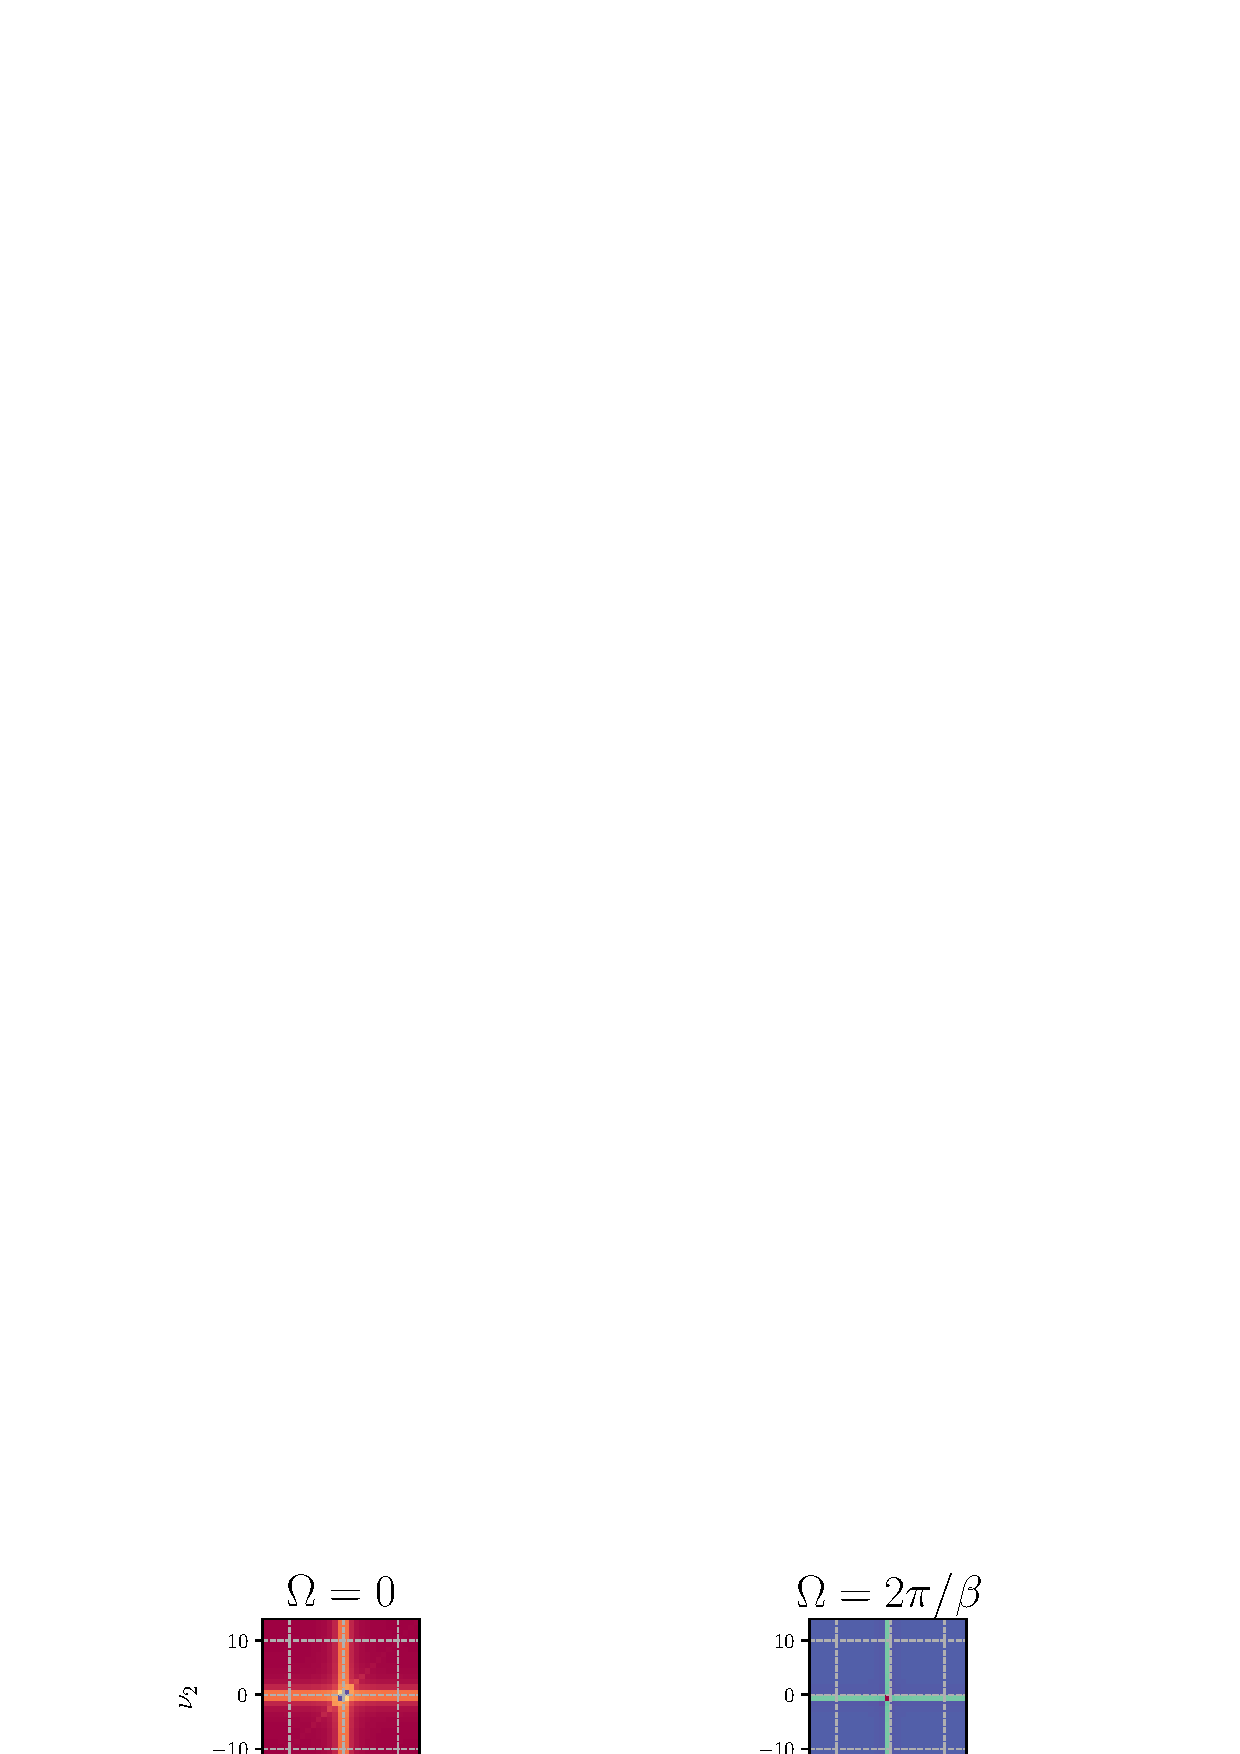
\includegraphics[width=\textwidth]{images/PL_all.png}
\vspace*{-2.0cm}
\caption{In the first three panels from the left, the charge channel $\mathcal{C}_{\bs{Q},\Omega}$ as in Eq.~\ref{pl:charge} is shown as 
a function of $\nu_1$ and $\nu_2$ for frequency $\Omega=0$, $\Omega=2\pi/ \beta$ and 
$\Omega=4\pi/ \beta$, respectively, for $\bs{Q}=(0,0)$. In the most right panel, the bubble $\Pi_{\bs{Q}=(0,0),\Omega}(\nu)$ is shown as a function of $\nu$ for 
$\Omega=0$, $\Omega=2\pi/ \beta$ and $\Omega=4\pi/ \beta$. All plots refer to parameters $T=1.0$, $t'=-0.32$, $x=0.375$ and $U=4$.  } 
\label{fig:perpladder}
\end{figure*}

In Fig.~\ref{fig:perpladder}, we show the charge channel as computed by Eq.~(\ref{pl:charge}) for different $\Omega$, $\bs{Q}=(0,0)$ as a function of $\nu_1$ and $\nu_2$, 
for $T=t$, $t'=-0.32t$, $U=4t$ and $x=0.375$.
We consider such a high temperature due to the above-mentioned overestimation of the fluctuations within RPA. 
The frequency structure in Fig.~\ref{fig:perpladder} for $\Omega=2\pi/ \beta$ is very similar to the one shown in Fig.~\ref{fig:freqplot}. 
The simple diagrams considered here reproduce the position of the main structures, as well as the correct sign of the charge channel. 
This is true also for the other bosonic Matsubara frequency shown here, for which we do not report the fRG results. 
Furthermore, upon lowering the temperature the charge channel diverges also for other finite bosonic Matsubara frequencies, while it does not diverge for $\Omega=0$.
From this we conclude that the diagrams described here are responsible for the frequency structure of the charge channel observed in fRG. 

To understand why the divergence appears for a finite frequency $\Omega$, we notice that in Eq.(\ref{pl:charge}) the $\Omega$ dependence 
appears only through the bubble $\Pi_{\bs{Q},\Omega}(\nu)$. The frequency summed particle-hole bubble obeys the following relation:  
\begin{equation}
	\Pi_{\bs{Q}\rightarrow(0,0),\Omega} = \frac{1}{\beta} \sum_{\nu} \Pi_{\bs{Q}\rightarrow(0,0),\Omega}(\nu) = C \delta_{\Omega,0},
\label{pl:sumrule}
\end{equation}
where $C$ is a constant that, at low temperature, approaches the density of states at the Fermi level.
In the rightmost panel of Fig.~\ref{fig:perpladder}, we show the bubble $\Pi_{\bs{Q}=(0,0),\Omega}(\nu)$ as a function of $\nu$ for different values of $\Omega$.
We note that it has a large negative peak for $\Omega=2\pi/ \beta$.
This is due to the property (\ref{pl:sumrule}): the summed 
bubble must vanish for $\Omega \neq 0$, hence a large negative value is needed to cancel the positive contributions at large frequency. 
%An argument based on the discontinuity of the bubble, Eq.~(\ref{pl:sumrule}) is also mentioned in Ref. \onlinecite{Stepanov2016}, to justify a possibly related non monotonous behavior of the retarded interaction .
We have thus identified the origin of the frequency structure observed in the charge channel, which seems to be quite general and arising from simple diagrams. 

Including the self-energy in the calculation of the bubble,   Eq.~(\ref{pl:sumrule}) does not evaluate to a $\delta$-function anymore, and the difference between the summed bubble at vanishing frequency and for frequency $2\pi T$ is diminished. 
This is probably the reason why the inclusion of the self-energy feedback is sufficient to avoid the divergence of the charge channel.     

%All these considerations suggest that the divergence of the charge channel is rather an artefact of fRG without self-energy, arising from a lack of consistence between the vertex and the Green's function in the flow equations. 
%In the next section we further substanciate this conclusion, by explaining the mathematical origin of the feature. 
%The self-energy has qualitative and quantitive effects on the flow equations: quantitively 
\subsection{Self energy analysis}
We discuss here the frequency and momentum dependence of the self energy. 
In Fig.~\ref{fig:selffermi0975}  we show the frequency dependence of the imaginary part of the self-energy for $U=4t$, $T=0.08t$,  $t'=-0.32t$ and doping $x=0.025$. 

This spread between the maximal and minimal self-energy at each frequency is rather small, indicating that the self-energy did not develop a large momentum dependence even when the vertex reached the critical scale. 
For all the momenta, the self-energy shows a Fermi-liquid like behavior (at finite temperature). 
In this situation one would expect the antinodal region to be more affected by correlation effects. 
However, we can only see a slight increase of the (absolute value of) self energy in this region. 
At the temperature that we are considering, we do not observe a tendency towards the opening of a momentum selective gap. 

In Fig.~\ref{fig:selffermi0600} we show the imaginary part of the self-energy for a larger doping $x=0.400$. For these parameters the incommensurability reaches its maximal value  $\delta=1.13$. 
As in the previous case, we do not see much momentum differentiation.

The self-energy enters directly in the calculation of the momentum resolved occupation through the Green's function, already discussed above, and shown in  Figs.~\ref{fig:occ975} and~\ref{fig:occ600}.
In the bottom panels of these figures,  we show how the occupation evolves along two different cuts in the Brillouin zone.
The two cuts are shown by arrows in the inset, and cross, respectively,  the \textit{nodal} and \textit{antinodal} regions.
The occupation drop is sharper along the main diagonal, and the self-energy affects more the occupation along the nodal cut.
For doping $x=0.4$ the broadening of the Fermi surface, already larger at the non interacting level, is further enhanced by the self-energy.

To study further the difference between nodal and antinodal regions in the iAF case, we studied the quasiparticle weight\cite{Abrikosov1963,Metzner2012} $\mathcal{Z}_{\bs{k}}$, and the decay rate $\gamma_{\bs{k}}$.
Instead of relying on analytical continuation, we have extracted the parameters directly from the imaginary axis data.
To do so we have fitted the first few frequencies of the imaginary part of the self-energy with a polynomial of degree $l$: $\mathrm{Im}\Sigma(\bs{k},i\nu)\approx a_0(\bs{k})+a_1(\bs{k})\nu+...+a_l(\bs{k})\nu^l$ and we identified $\gamma_{\mathbf{k}}=a_0(\bs{k})$, $\mathcal{Z}_{\bs{k}}= \frac{1}{1-a_1(\bs{k})}$.
The procedure only works if the temperature is small enough, and if the frequencies used for the fitting are not too high. We checked that the results were stable by changing the number of frequencies and the order of the polynomial used for the fit. 
The results are shown in Fig.~\ref{fig:zetaandgamma}, where the value of $\mathcal{Z}_{\bs{k}}$ and $\gamma_{\bs{k}}$ is plotted against the angle $\theta$ along the Fermi surface, $\theta=0$ corresponding to the antinodal point and $\theta=\pi/4$ to the nodal one. 
The variation of the quasiparticle weight along the Fermi surface is extremely small with $\mathcal{Z}$ assuming values between $0.754$ and $0.760$. 
On the other hand the relative variation of the decay rate $\gamma$ along the Fermi surface is larger, varying from $\gamma\approx 0.056t$ and $\gamma \approx 0.082t$. These values are comparable with the temperature $T=0.08t$. 
We conclude that at the critical scale, the system still has coherent quasiparticles along all the Fermi surface, with a higher decay rate in the antinodal region. This is consistent with the observations of Ref.~\cite{Rohe2005}, where it is shown that non Fermi liquid behavior of the self-energy is observed only very close to the critical temperature and in the immediate vicinity of the hot spots. \emph{I did not really know where to add the citation, we can expand commenting that it is Wick-ordered?}  
\begin{figure}
\includegraphics[width=0.50\textwidth]{images/Self_Im_occ0975.png}
\caption{Frequency dependent self-energy for $U=4t$, $T=0.08t$, $t'=-0.32t$, $x=0.025$.
Red symbols refer to the Fermi surface momentum in the antinodal direction,  blue symbols to the Fermi surface momentum on the diagonal, while  green symbols refer to a momentum on the Fermi-surface between these two extremes. 
The location of the $\mathbf{k}$-point in the Brillouin zone is color coded in the inset.  
The position of all the patching points taken into account for the self-energy is shown as black circles in the top row of Figs.~\ref{fig:occ975} and ~\ref{fig:occ600}, and does not change during the flow.
The shaded area highlights the region between the maximal and minimal value of the self-energy for each frequency. }
\label{fig:selffermi0975}
\end{figure}


\begin{figure}
\includegraphics[width=0.50\textwidth]{images/Self_Im_occ0600.png}
\caption{Frequency dependent self-energy for $U=4t$, $T=0.08t$, $t'=-0.32t$, $x=0.4$.
Red symbols refer to the Fermi surface momentum in the antinodal direction,  blue symbols to the Fermi surface momentum on the diagonal, while  green symbols refer to a momentum on the Fermi-surface between these two extremes. 
The location of the $\mathbf{k}$-point in the Brillouin zone is color coded in the inset.  
The position of all the patching points taken into account for the self-energy is shown as black circles in the top row of Figs.~\ref{fig:occ975} and ~\ref{fig:occ600}, and does not change during the flow.
The shaded area is the region between the maximal and minimal value of the self-energy for each frequency.}
\label{fig:selffermi0600}
\end{figure}

\begin{figure}
\includegraphics[width=0.5\textwidth]{images/z_and_gamma975.png}
\caption{Quasiparticle weight $\mathcal{Z}_{\bs{k} }$ and decay rate $\gamma_{\bf{k}}$ as function of the angle $\theta$. 
The values on the left axis refer to the quasiparticle weight. The values on the right axis refer to the decay rate.}
\label{fig:zetaandgamma}
\end{figure}
